\section{Service Layer Architecture}

The Service Layer serves as the backbone of the Library Management System, orchestrating business logic and coordinating operations between different system components. This layer implements SOLID principles and integrates multiple design patterns to ensure flexibility, scalability, and maintainability.

\subsection{Service Layer Overview}

The Service Layer acts as an intermediary between the Presentation Layer and Domain Layer, encapsulating core business functionality:

\begin{itemize}
	\item \textbf{Business Logic Execution}: Enforcing library policies and operational rules
	\item \textbf{Transaction Orchestration}: Managing multi-step operations atomically
	\item \textbf{Component Integration}: Coordinating interactions between system modules
	\item \textbf{Security Services}: Providing authentication and authorization mechanisms
	\item \textbf{Event Management}: Handling system notifications and observer patterns
	\item \textbf{Data Coordination}: Managing persistence operations across entities
\end{itemize}

\subsection{Library Manager - Centralized Business Coordinator}

The LibraryManager class represents the core of the Service Layer, implementing multiple design patterns for robust system management:

\subsubsection{Singleton Pattern Implementation}

LibraryManager follows the Singleton pattern to ensure:
\begin{itemize}
	\item Single point of control for library operations
	\item Consistent state management across the application
	\item Thread-safe instance management
	\item Global access to library functionality
\end{itemize}

% % TODO: Add LibraryManager Singleton UML diagram
% \begin{figure}[H]
%     \centering
%     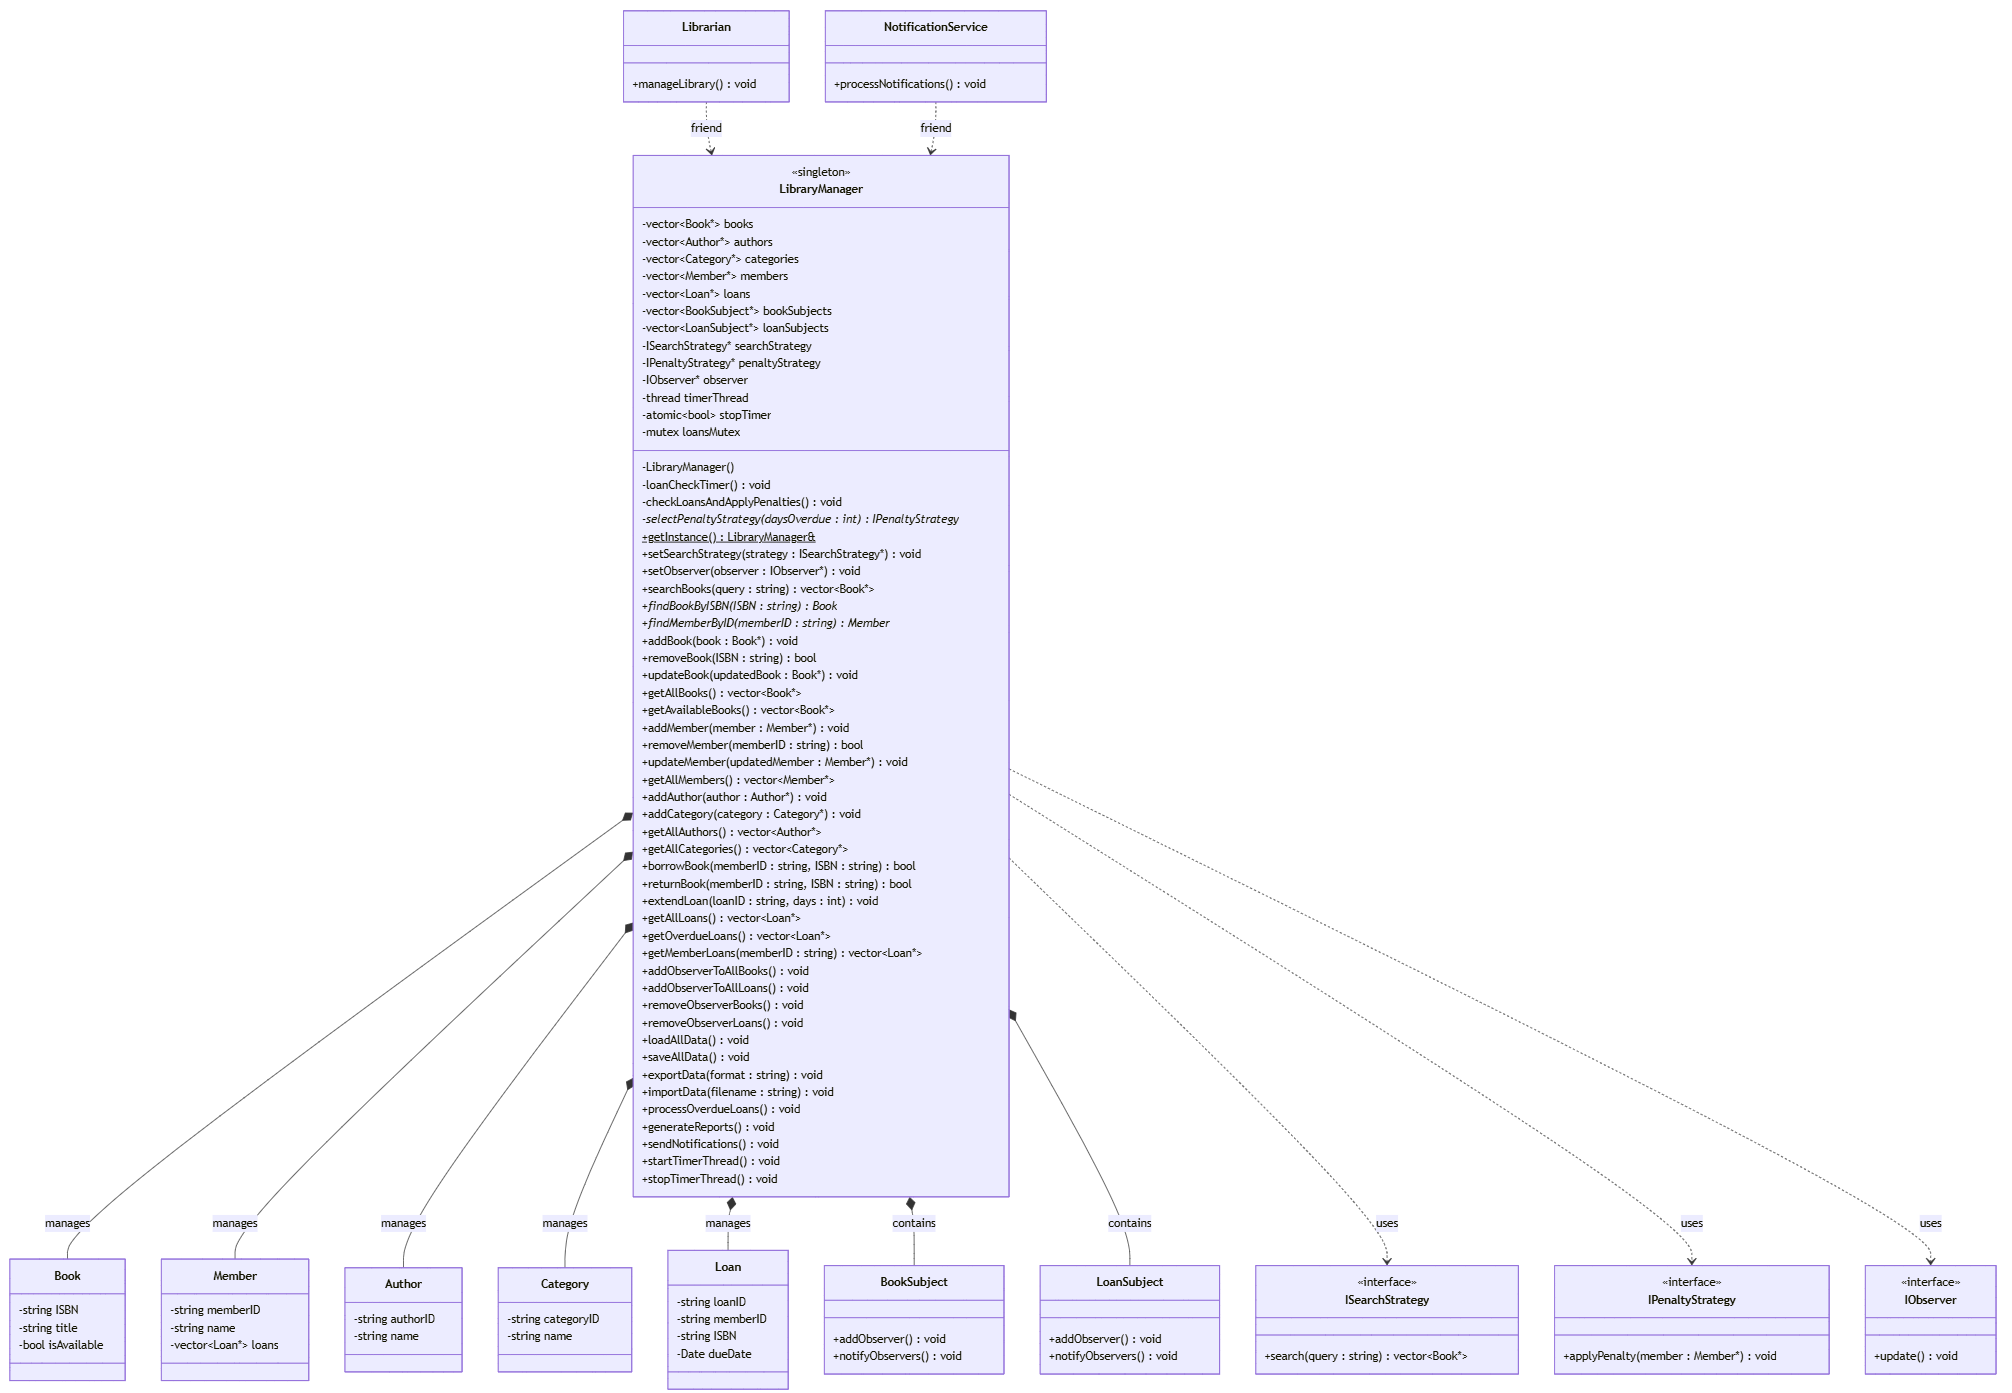
\includegraphics[width=0.8\textwidth]{figures/singleton_pattern.png}
%     \caption{LibraryManager singleton implementation showing getInstance\(\) method and private constructor}
%     \label{fig:library-manager-singleton}
% \end{figure}

\subsubsection{Facade Pattern Integration}

LibraryManager acts as a unified facade providing simplified access to complex subsystems:

\begin{itemize}
	\item \textbf{Book Management}: addBook(), findBook(), loadBooksIntoLibrary()
	\item \textbf{Member Operations}: addMemberToSystem(), findMember(), loadMembersFromCSV()
	\item \textbf{Loan Processing}: borrowBook(), returnBook(), loadLoansFromCSV()
	\item \textbf{Search Coordination}: searchBooks() with strategy pattern integration
	\item \textbf{Notification Management}: Observer attachment and event distribution
\end{itemize}

% % TODO: Add Facade Pattern diagram showing LibraryManager coordinating subsystems
% \begin{figure}[H]
%     \centering
%     \textbf{[TODO: LibraryManager Facade Pattern Diagram]}
%     \caption{LibraryManager facade coordinating Book, Member, Loan, and Notification subsystems}
%     \label{fig:library-manager-facade}
% \end{figure}

\subsection{Authentication Manager - Security Services}

The AuthenticateManager provides comprehensive user identity and access management:

\subsubsection{Core Authentication Features}
\begin{itemize}
	\item User registration with role-based assignment
	\item Credential verification and session management
	\item CSV-based user storage with data validation
	\item Basic password security enforcement
\end{itemize}

\subsubsection{Role-Based Access Control}
The system implements a hierarchical permission structure:
\begin{itemize}
	\item \textbf{Member}: Book borrowing and profile management
	\item \textbf{Librarian}: Administrative functions and system management
\end{itemize}

% TODO: Add Authentication Manager architecture diagram
\begin{figure}[H]
	\centering
	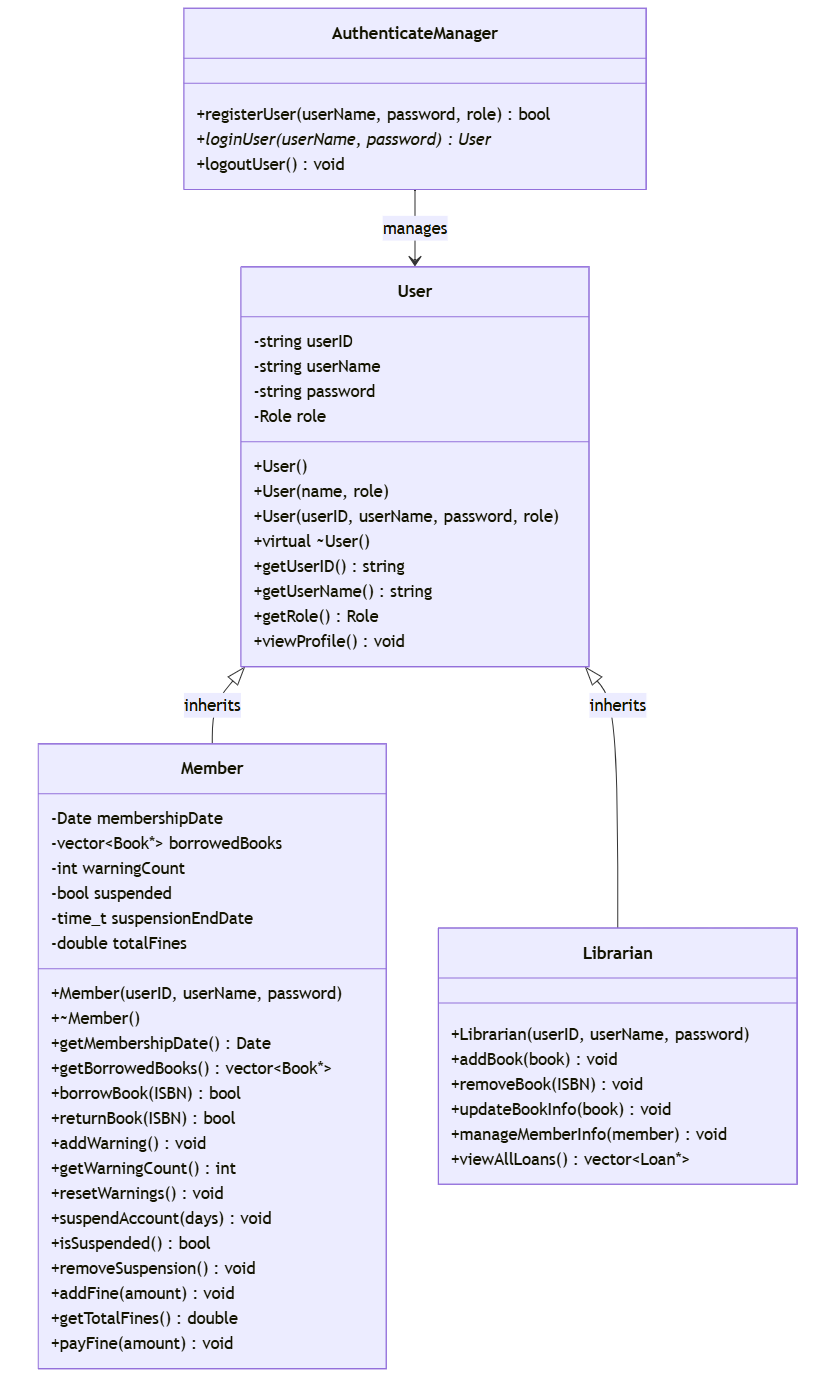
\includegraphics[width=0.5\textwidth]{figures/authenticate.png}
	\caption{AuthenticateManager coordinating User, Member, and Librarian authentication}
	\label{fig:auth-manager-service}
\end{figure}

\subsection{Notification Service - Event-Driven Communication}

The NotificationService implements the Observer pattern for real-time system communication:

\subsubsection{Service Architecture}
\begin{itemize}
	\item \textbf{Event Processing}: Handling book and loan status changes
	\item \textbf{Observer Coordination}: Managing MemberObserver and LibrarianObserver instances
	\item \textbf{Delivery Mechanisms}: Console notifications and file-based logging
	\item \textbf{Due Date Monitoring}: Automated overdue loan notifications
\end{itemize}

\subsubsection{Notification Categories}
\begin{itemize}
	\item Book availability changes
	\item Loan status updates and due date reminders
	\item Overdue notifications for library staff
	\item System alerts and administrative notifications
\end{itemize}

% TODO: Add Notification Service Observer pattern diagram
\begin{figure}[H]
	\centering
	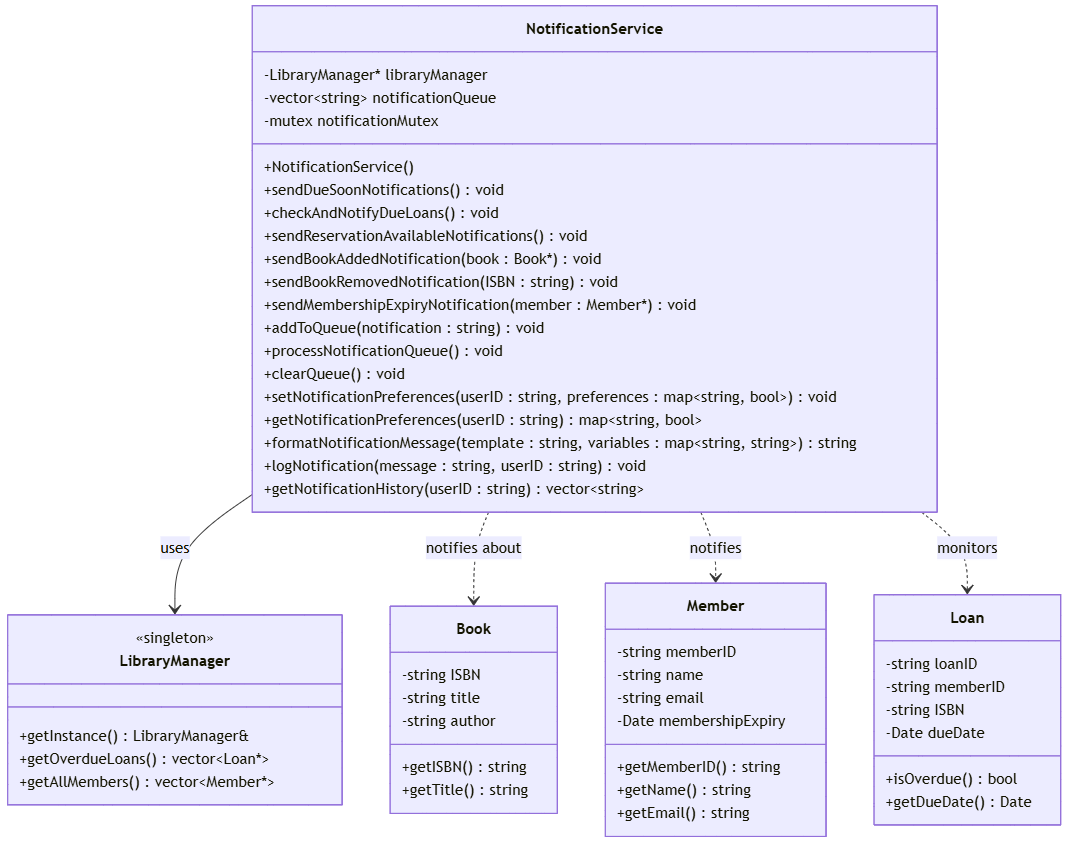
\includegraphics[width=0.8\textwidth]{figures/notification_service.png}
	\caption{NotificationService coordinating BookSubject, LoanSubject, and Observer implementations}
	\label{fig:notification-service}
\end{figure}

\subsection{Data Management Service - Persistence Coordination}

The Data Management Service ensures reliable data persistence and integrity:

\subsubsection{CSV Handler Integration}
\begin{itemize}
	\item \textbf{Data Persistence}: CSV-based storage with atomic operations
	\item \textbf{Validation Services}: Input validation and data integrity checking
	\item \textbf{Backup Management}: Automatic backup creation before modifications
	\item \textbf{Cross-Platform Compatibility}: Human-readable data format support
\end{itemize}

\subsubsection{Transaction Management}
\begin{itemize}
	\item Coordinated save operations across multiple entities
	\item Rollback capabilities for data consistency
	\item Concurrent access protection through file locking
\end{itemize}

% TODO: Add Data Management Service architecture diagram
\begin{figure}[H]
	\centering
	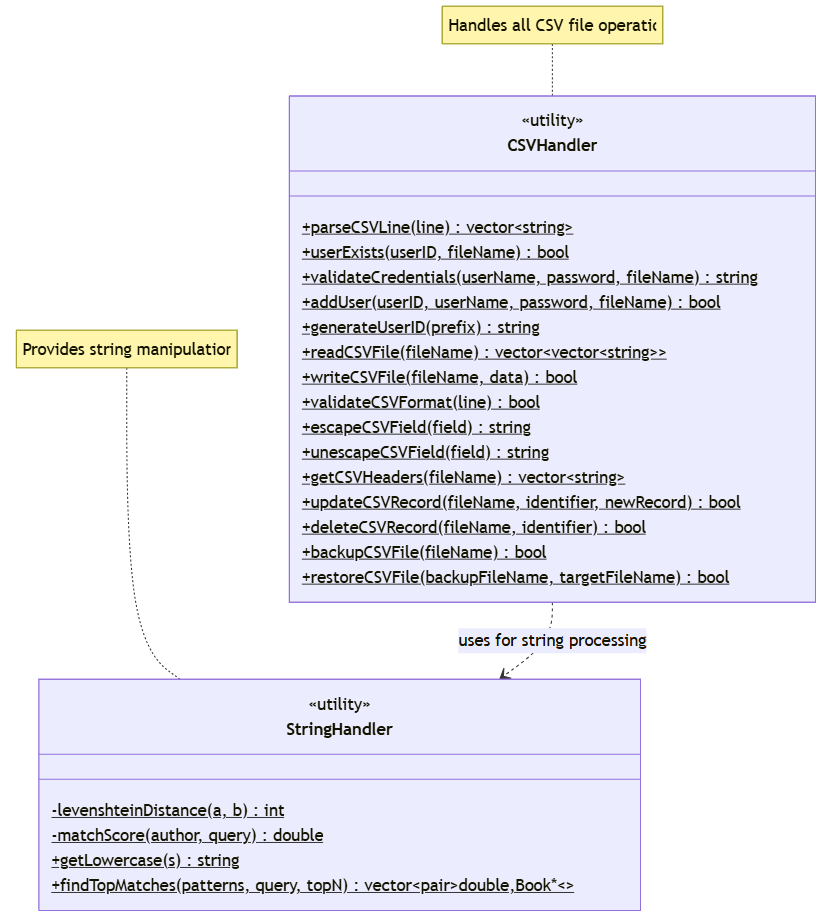
\includegraphics[width=0.8\textwidth]{figures/string_handler.png}
	\caption{CSVHandler and data persistence services coordination within the Service Layer}
	\label{fig:data-management-service}
\end{figure}

\subsection{Service Layer Benefits and Design Principles}

\subsubsection{SOLID Principles Implementation}
\begin{itemize}
	\item \textbf{Single Responsibility}: Each service has a focused, well-defined purpose
	\item \textbf{Open/Closed}: Services extensible through strategy and observer patterns
	\item \textbf{Liskov Substitution}: Strategy implementations interchangeable at runtime
	\item \textbf{Interface Segregation}: Focused interfaces for specific service contracts
	\item \textbf{Dependency Inversion}: Services depend on abstractions, not concretions
\end{itemize}

\subsubsection{Pattern Integration Benefits}
\begin{itemize}
	\item \textbf{Singleton + Facade}: Centralized and simplified system access
	\item \textbf{Observer + Strategy}: Flexible notification with pluggable algorithms
	\item \textbf{Service Coordination}: Clean separation of concerns with loose coupling
	\item \textbf{Maintainability}: Clear architecture supporting future enhancements
\end{itemize}

% % TODO: Add Service Layer integration overview diagram
% \begin{figure}[H]
%     \centering
%     \textbf{[TODO: Service Layer Integration Overview]}
%     \caption{Complete Service Layer architecture showing all services and their interactions}
%     \label{fig:service-layer-overview}
% \end{figure}

\section{Application Walkthrough and Usage}
\label{sec:walkthrough}

This section demonstrates the system in action by walking through its primary use cases. For each key feature, we provide a description of the user interaction, a UML Sequence Diagram to illustrate the technical flow of method calls between objects, and screenshots to showcase the console-based user interface.
